\documentclass{beamer}

\usepackage{url}

\newcommand\vs{\vspace{\baselineskip}}

\newcommand\titlecite{
{\em Of all natural systems, living matter preserves inscribed in its organization the largest amount of its own past history .... no other system is better}
 aufgehoben:
{\em constantly abolished and simultaneously preserved.}
\cite{PaulingZuckerkandl63}}

\newcommand\presentation[1]{ \section*{PRESENTATION: #1} }



% workaround for beamer bug
\providecommand\thispdfpagelabel[1]{}  % workaround

% presentation
\mode<presentation>
{
  \usetheme{Warsaw}
  % or ...

  \setbeamercovered{transparent}
  % or whatever (possibly just delete it)
}


\usepackage[english]{babel}
% or whatever

\usepackage[latin1]{inputenc}
% or whatever

\usepackage{times}
\usepackage[T1]{fontenc}
% Or whatever. Note that the encoding and the font should match. If T1
% does not look nice, try deleting the line with the fontenc.


\title[Dirichlet process] % (optional, use only with long paper titles)
{Dirichlet Process}

\subtitle
{or, $K$-means without $K$} % (optional)

\author% [Holmes] (optional, use only with lots of authors)
{I.~Holmes} % \inst{1} \and S.~Another\inst{2}
% - Use the \inst{?} command only if the authors have different
%   affiliation.

\institute[University of California, Berkeley] % (optional, but mostly needed)
{
%  \inst{1}%
  Department of Bioengineering\\
  University of California, Berkeley}
% - Use the \inst command only if there are several affiliations.
% - Keep it simple, no one is interested in your street address.

\date%[Short Occasion] % (optional)
{Spring semester}

\subject{Talks}
% This is only inserted into the PDF information catalog. Can be left
% out. 



% If you have a file called "university-logo-filename.xxx", where xxx
% is a graphic format that can be processed by latex or pdflatex,
% resp., then you can add a logo as follows:

% \pgfdeclareimage[height=0.5cm]{university-logo}{university-logo-filename}
% \logo{\pgfuseimage{university-logo}}



% Delete this, if you do not want the table of contents to pop up at
% the beginning of each subsection:
\AtBeginSubsection[]
{
  \begin{frame}<beamer>{Outline}
    \tableofcontents[currentsection,currentsubsection]
  \end{frame}
}


% If you wish to uncover everything in a step-wise fashion, uncomment
% the following command: 

%\beamerdefaultoverlayspecification{<+->}


\begin{document}

\begin{frame}
  \titlepage
\end{frame}

\begin{frame}{Outline}
  \tableofcontents
  % You might wish to add the option [pausesections]
\end{frame}

\section{How Bayesian can $K$-means be?}

\begin{frame}{$K$-means (yet) again}

We presented $K$-means as a special case of the EM algorithm
\itemb
\item Model: \alert{mixture of Gaussians}
\item Parameters: Gaussian parameters
\item Missing data: cluster = mixture component
\item Counts: post.prob. of each component
\iteme

\vspace{\baselineskip}

Note that it's not Bayesian:
\[
\hat{\theta} = \argmax_{\theta} \sum_X P(X,Y|\theta)
\]
For example, there's no explicit prior on $\theta$...

\end{frame}


\begin{frame}{$K$-means made (a bit) Bayesian}

Let's put a prior on $\theta$:
\begin{eqnarray*}
\hat{\theta} & = & \argmax_{\theta} P(\theta|Y) \\
& = & \argmax_{\theta} \sum_X \frac{P(X,Y|\theta) P(\theta)}{P(Y)} \\
& = & \argmax_{\theta} \sum_X P(X,Y|\theta) P(\theta)
\end{eqnarray*}

OK so far, but a good Bayesian might also be interested in more details about the posterior distribution e.g. the moments
\[
\langle \theta^n \rangle_{P(\theta|Y)}
\]

\end{frame}

\begin{frame}{$K$-means made (a bit) Bayesian}

What should the prior be?

The ``easy'' choice is a conjugate Normal-gamma prior.
Suppose each mixture component has mean $\mu$ and precision $\tau$, and generates samples $y$, then
\begin{eqnarray*}
\tau & \sim & \mbox{Gamma}(\alpha,\beta) \\
\mu\ |\ \tau & \sim & \mbox{Normal}(\epsilon,(\lambda \tau)^{-1/2}) \\
y\ |\ \tau, \mu & \sim & \mbox{Normal}(\mu,\tau^{-1/2})
\end{eqnarray*}

This leads to straightforward modifications of our EM algorithm
 ($\alpha$, $\beta$, $\lambda$ and $\epsilon$ play the role of pseudocounts).

\end{frame}

\begin{frame}{$K$-means made (more) Bayesian}

The Good Bayesian is not content with $\hat{\theta}$.

The Good Bayesian wants $P(\theta|Y)$, and maybe $P(X|Y)$ too.

\itemb
\item We can use Gibbs sampling for this
\item Note that, given $X$ (cluster assignments), we can compute
\[
P(Y|X) = \int P(\theta)P(Y|X,\theta) d\theta
\]
and hence $P(\theta|X,Y)$.
\item Therefore we only need to sample cluster assignments
\iteme

\end{frame}


\begin{frame}{Complete Gibbs sampler for $K$-component mixture}

Joint likelihood of data and cluster assignments (assuming uniform mixture weights)
\begin{eqnarray*}
P(X,Y) = P(X) P(Y|X,\theta) = \left( \frac{1}{K} \right)^N \prod_{k=1}^K \int P(\theta_k) \left( \prod_{i: X_i = k} P(Y_i|\theta_k) \right) d\theta
\end{eqnarray*}

Gibbs-sampling algorithm:
\itemb
\item Remove a random datapoint from its cluster
\item Calculate the likelihood for placing the datapoint in any existing cluster
\item Randomly sample the datapoint's new cluster from these likelihoods
\iteme

\end{frame}



\begin{frame}{Why $K$-means can never be truly Bayesian}

\itemb
\item \alert{We Still Need To Know $K$} (the number of mixture components)
\item Of course we can introduce a prior $P(K)$
\item However, doing MCMC over $K$ is tricky, because changing $K$ changes the dimensionality of $\theta$
\item There are ways around this, e.g. \alert{reversible-jump MCMC}
\item The Dirichlet Process is (arguably) a more elegant solution
\iteme

\end{frame}

\begin{frame}{$K$-multinomials: motivation}

\itemb
\item Generative model for clustering is a mixture distribution
 \itemb
 \item First, randomly choose a component
 \item Next, use that component to generate your data
 \iteme
\item Before going further, it is useful to have a physical analogy for each component distribution
\itemb
\item Physical analogy for a Gaussian is possible, but...
\item Physical analogy for a multinomial is much easier:
\iteme
\iteme

\centerline{
  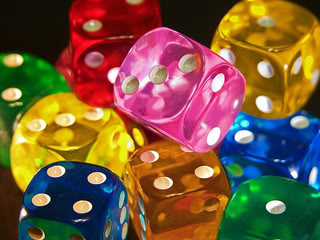
\includegraphics[height=.5\textheight]{ColorfulDice3D.jpg}
  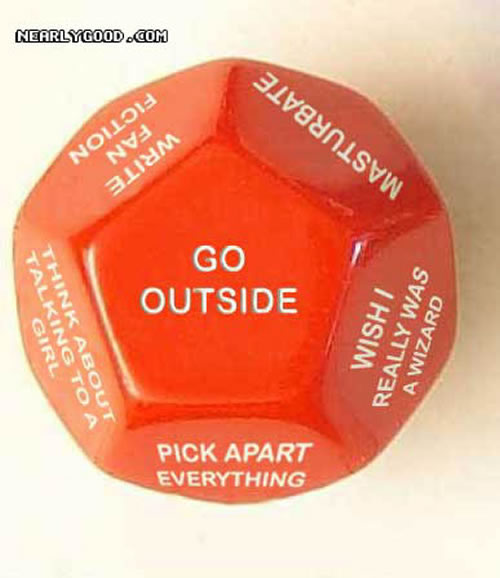
\includegraphics[height=.5\textheight]{WarcraftFanDice.jpg}
}

\end{frame}

\begin{frame}{$K$-multinomials vs $K$-Gaussians}

\itemb
\item Mixture of $K$ Gaussians $\to$ Mixture of $K$ multinomials
\item Physical analogy:
\itemb
 \item Bag of (loaded) dice, each $D$-sided
 \item Pick a die from the bag
 \item Roll it $N$ times; count outcomes
 \item This corresponds to one $D$-dimensional datapoint
\iteme
\item EM algorithm is actually quite similar (even simpler)
 \itemb
 \item Each casino punter picks a die from the bag
  \inone{Rolls it $N$ times, then puts it back in the bag}
 \item Missing data ($X$) specifies which die each punter chose
 \item Observed data ($Y$) are the vectors of $D$ counts for each punter
 \item Parameters ($\theta$) are the probabilities for each of the dice
 \item Likelihood $P(X,Y|\theta)$ is a bit different from the Gaussian...
 \inone{\alert{Exercise: derive the EM algorithm for $K$-multinomials}}
 \iteme
\iteme

\end{frame}


\begin{frame}{$K$-multinomials: the Bayesian version}

\itemb
\item Again, we need a prior for each model component $\theta$
\item Again, an easy choice is the conjugate to $P(y|\theta)$
 \inone{conjugate to the multinomial = the \alert{Dirichlet distribution}}
\item Analogy: the Dirichlet represents a \alert{dice-making machine}
 \inone{For $D=2$, the Beta distribution, a \alert{coin-minting machine}}
\item Note that Dirichlet distribution $\neq$ Dirichlet process
 \itemb
 \item We could use (Gaussian,Normal-Gamma) instead of (Multinomial,Dirichlet)
 \item DP and DD {\em are} related, but in a somewhat technical sense
 \iteme
\item Key point is that it's useful to be able to directly compute
\[
P(Y) = \int_{\theta} P(Y|\theta) P(\theta) d\theta
\]
for an individual component $\theta$ generating datapoints $Y$.
\iteme

\end{frame}


\section{Infinite-component mixtures}

\begin{frame}{Infinite-component mixtures}

The general idea is that, instead of trying to estimate the number of mixture components $K$,
we will assume that there are an \alert{infinite} number of components.

\end{frame}

\begin{frame}{What happens if we set $K = \infty$?}

\itemb
\item With $K = \infty$, there are an infinite number of datapoint$\to$component assignments
 \itemb
 \item Infinite number of dice in the bag (or ``on the bench''?)
 \item So, infinite number of possible explanations
 \iteme
\item Suppose $X = (x_1, x_2, x_3, x_4, x_5)$ are the dice used by the first five consecutive punters
\item In some sense, $(5, 2, 5, 10, 2)$ is the same as $(104, 300, 104, 2095, 300)$
\item All we really care about is the \alert{partition} --- not the exact labeling. The number of partitions is always finite.
 \inone{Both the above cases have the partition \\ $\{ (1\ 3) (2\ 5) (4) \}$}
\item Note that the problem of \alert{identifiability} arises even with finite $K$. Only the partition matters, really...
\iteme

\end{frame}

\begin{frame}{The Dirichlet process}

\itemb
\item The DP can be conceived of as an infinite mixture, $K=\infty$
 \itemb
 \item But not with uniform component weights!
 \item Some dice are more likely to be drawn from the bench
 \item Otherwise no two punters would never use the same die
 \iteme
\item There are several (equivalent) ways to define the DP:
 \itemb
 \item The \alert{stick-breaking construction}
\inone{This is the ``infinite-component mixture'' view}
 \item The \alert{Chinese Restaurant process}
\inone{This emphasizes the partitions, rather than the components}
 \item The \alert{formal definition}
\inone{This is where Dirichlet distributions come in}
 \iteme
\item A common application is to use MCMC to sample partitions
\iteme

\end{frame}

\begin{frame}{Parameters of the Dirichlet process}

The DP has two parameters:

\itemb
\item A \alert{concentration parameter}, $\alpha$, that drives the number of clusters, via the \alert{Chinese Restaurant Process} (CRP)
 \itemb
 \item Not fixed like $K$, but analogous
 \item High $\alpha$ means lots of clusters
 \item Canonical value is $\alpha=1$
 \iteme
\item A \alert{base distribution}, $G_0(\theta)$, that is auxiliary to the CRP
 \itemb
 \item This represents the prior on parameters for an individual component (cluster)
 \item Typical choice: conjugate to the component likelihood
 \itemb
  \item So, in our casino example, it is a Dirichlet distribution (conjugate to multinomial)
  \item For the DP version of $K$-means, it would be the Normal-Gamma (conjugate to Gaussian)
 \iteme
 \iteme
\iteme

\end{frame}


\begin{frame}{Chinese Restaurant Process}

The usual formulation:
\itemb
\item Chinese restaurant with infinite tables, each infinitely large
\item Customer \#1 enters and sits at a table
\item Customer \#2 sits at the same table with probability $1/(1+\alpha)$, or a new table with $P=\alpha/(1+\alpha)$
\item This continues: customer \#$(n+1)$ sits at a $k$-person table with $P=k/(n+\alpha)$ and a new table with $P=\alpha/(n+\alpha)$
\iteme

With $n$ customers in the restaurant, let $b$ denote the set of customers at a particular table and $B_n = \{ b \}$ the set of all occupied tables.
($B_n$ is a \alert{partition} of the $n$ customers.)
Then
\[
P(B_n = B|\alpha) = \frac{\Gamma(\alpha) \alpha^{|B|}}{\Gamma(\alpha+n)} \prod_{b \in B} \Gamma(|b|)
\]

Can think of $\alpha$ as the number of ``imaginary friends''...

\end{frame}


\begin{frame}{Derivation of the partition probability}

Let $B_{n-1}$ be the partition when customer $n$ enters the restaurant.

Let $b_n$ be the random table joined by customer $n$.

\[
P(b_n=b|b_1,\ldots,b_{n-1}) = \left\{ \begin{array}{ll}
\frac{\alpha}{\alpha + n - 1} & \mbox{if $b_n \notin B_{n-1}$ (new table)} \\
\frac{|b|}{\alpha + n - 1} & \mbox{if $b_n \in B_{n-1}$ (existing table)}
\end{array} \right.
\]

This leads to the stated form of $P(B_n)$
\begin{eqnarray*}
\lefteqn{P(B_n = B)} \\
& = & \frac{\alpha^{|B|}}{(\alpha+n-1) \times (\alpha+n-2) \times \ldots \times (\alpha+1) \times \alpha}
 \prod_{b \in B} (|b|-1)!
\end{eqnarray*}


\end{frame}




\begin{frame}{The CRP and the Dirichlet Process}

Now think of dice-making machines:
\itemb
\item Restaurant is also a casino, owns a dice-making machine
\item There is a die on every table (all from the same machine)
\item Each punter chooses a table sociably (just like the CRP) and then rolls the die at that table
\item Thus, punter \#2 re-uses first die with $P=1/(1+\alpha)$, or a new die with $P=\alpha/(1+\alpha)$
\item This continues: the $(n+1)$'th punter uses a new die with probability $P=\alpha/(n+\alpha)$; otherwise, they pick one of the previous punters at random and re-use that punter's die
\iteme

Thus, we use the CRP (with parameter $\alpha$) to define a prior on the partitioning of the data to components,
and $G_0$ (which here is a Dirichlet distribution) to sample the parameter used by each component.

\end{frame}








\begin{frame}{The partition-conditioned likelihood}

Given a particular partition, $B$, we can write down the likelihood.

Let the data be $Y = \{ Y_1 \ldots Y_n \}$ and let $Y^{(b)} = \{ Y_n: n \in b \}$ be the subset associated with a particular block of the partition.

\[
P(Y|B,G_0) = \prod_{b \in B} \int G_0(\theta) P(Y^{(b)}|\theta) d\theta
\]

This is simplified if $G_0$ is conjugate to the likelihood $P(Y|\theta)$.

\end{frame}


\begin{frame}{Properties of the CRP}

With $n$ customers in the restaurant, let $b$ denote the set of customers at a particular table and $B_n = \{ b \}$ the set of all occupied tables.
\[
P(B_n = B|\alpha) = \frac{\Gamma(\alpha) \alpha^{|B|}}{\Gamma(\alpha+n)} \prod_{b \in B} \Gamma(|b|)
\]
In the special case of $\alpha=1$
\[
P(B_n = B|\alpha = 1) = \frac{\prod_{b \in B} (|b|-1)!}{n!}
\]

Note that $P(B_n)$ is \alert{exchangeable}, i.e. invariant to permutations of the customers.
This is a useful property because it means we can remove any customer, and reintroduce them as if they were the last one to enter the restaurant.
This is effectively how we do Gibbs-sampling under the DP.

\end{frame}


\begin{frame}{Gibbs sampling reviewed}

Recall the core idea of Gibbs sampling:
\itemb
\item We want to sample from a multivariate probability distribution $P({\bf x}) = P(x_1,x_2,x_3,\ldots x_N)$
\item We seek a Markov chain with transition probability $Q({\bf x}'|{\bf x})$ and equilibrium $P({\bf x})$, satisfying \alert{detailed balance}
\[
P({\bf x}) Q({\bf x}'|{\bf x}) = P({\bf x}') Q({\bf x}|{\bf x}')
\]
\item We achieve this by sampling exactly from the marginal distribution of one of the $N$ variables, given all the others
\begin{eqnarray*}
Q_k({\bf x}'|{\bf x}) & = & P(x'_k | \{ x_n : n \neq k \}) \prod_{n \neq k} \delta(x'_n = x_n) \\
Q({\bf x}'|{\bf x}) & = & \sum_{k=1}^N \frac{1}{N} Q_k({\bf x}'|{\bf x})
\end{eqnarray*}
\iteme

\end{frame}

\begin{frame}{Complete Gibbs sampler for the DP}

Joint likelihood of data and partition
\[
P(Y,B|\alpha,G_0) = P(B|\alpha) P(Y|B,G_0)
\]

Gibbs-sampling algorithm:
\itemb
\item Remove a random datapoint from its cluster (block, table)
\item Calculate the likelihood for placing the datapoint in any existing cluster, as well as in its own new cluster
\item Randomly sample the datapoint's new cluster from these likelihoods
\iteme

\end{frame}



\begin{frame}{Stick-breaking construction of the CRP}

\itemb
\item Coin-making machine produces coins $\sim \mbox{Beta}(1,\alpha)$
\item There is a coin on each table
\item The tables are numbered ($1, 2, 3 \ldots$)
\item Visit the tables in order, flipping coins until you get a ``Heads''
\item Sit at that table
\iteme

Notes:
\itemb
\item This gives the same marginal distribution of partitions as the CRP, if you integrate out the coin probabilities and sum out the table numbers
\iteme

\end{frame}


\begin{frame}{Why ``stick-breaking''?}

The more usual formulation is that instead of a series of coins with probabilities $p_1,p_2,p_3 \ldots$
we break a unit-length stick into successively shorter pieces, with the $n$'th piece having length
\[
\ell_n = p_n \prod_{k=1}^{n-1} (1 - p_k)
\]
The probability of sitting at the $n$'th table is $\ell_n$.

\end{frame}




\begin{frame}{Stick-breaking construction of the DP}

\itemb
\item Dice-making machine produces dice $\sim G_0$
\item Coin-making machine produces coins $\sim \mbox{Beta}(1,\alpha)$
\item There is a coin {\em and} a die on each table
\item The tables are numbered ($1, 2, 3 \ldots$)
\item Visit the tables in order, flipping coins until you get a ``Heads''
\item Pick the die on that table
\iteme

Notes:
\itemb
\item The resulting distribution over dice ($\theta$) shares many properties with the underlying machine ($G_0$),
but unlike $G_0$, it is a \alert{discrete} distribution ($G_0$ is \alert{continuous})
\item Equivalently: there is a finite probability of getting the exact same die twice (whereas the machine will {\bf never} produce two identical dice)
\iteme

\end{frame}



\begin{frame}{Formal definition of the DP}

For completeness...

\vspace{.5\baselineskip}

Let $G_0$ be a probability measure over some measurable space $(\Theta,{\cal B})$ and let $\alpha$ be a positive real number.

\vspace{.5\baselineskip}

A {\em Dirichlet Process}, DP$(\alpha,G_0)$, is the distribution of a random measure $G$ over $(\Theta,{\cal B})$
such that, for any partition $(A_1, A_2, \ldots, A_r)$ of $\Theta$, the finite-dimensional distribution of that partition according to $G$ is Dirichlet-distributed:
\[
(G(A_1),G(A_2) \ldots G(A_r)) \sim \mbox{Dirichlet}(\alpha G_0(A_1), \alpha G_0(A_2) \ldots \alpha G_0(A_r))
\]


\end{frame}



\section{Bioinformatic applications of the CRP}

\begin{frame}{CRP and DP in biology}

\itemb
\item P\'{o}lya Urn formulations of the CRP
\item Ewens' Sampling Formula
\item Machine learning (clustering, regression, \ldots)
\iteme

\end{frame}

\begin{frame}{P\'{o}lya Urn formulation}

The CRP itself (Hoppe, J of Math. Biol. 1984)
\itemb
\item Start with an urn containing
 \itemb
 \item one black ball of mass $\alpha$
 \item $n_k$ balls of color $k$ and unit mass
 \item Initially all the $n_k$ are zero (just one black ball)
 \iteme
\item Draw a ball from the urn, proportionally to its mass
 \itemb
 \item If it's black, replace it in the urn, together with a unit-mass ball of a new color
 \item If it's not black, replace it in the urn, together with a unit-mass ball of the same color
 \iteme
\item Note that the black ball is {\em ``ignored in describing the urn configuration since it is always present and merely a device for generating new labels''} (Hoppe)
\iteme

\end{frame}

\begin{frame}{P\'{o}lya Urn formulation}

The Gibbs sampler for the CRP
\itemb
\item The urn contains
 \itemb
 \item one black ball of mass $\alpha$
 \item $n_k$ balls of color $k$ and unit mass
 \iteme
\item Remove a (colored) ball from the urn and discard it
\item Draw a ball from the urn, proportionally to its mass
 \itemb
 \item If it's black, replace it in the urn, together with a unit-mass ball of a new color
 \item If it's not black, replace it in the urn, together with a unit-mass ball of the same color
 \iteme
\iteme

\end{frame}

\begin{frame}{Ewens's Sampling Formula}

Here (again) is the partition probability for $n$ customers
\[
P(B_n = B|\alpha) = \frac{\Gamma(\alpha) \alpha^{|B|}}{\Gamma(\alpha+n)} \prod_{b \in B} \Gamma(|b|)
\]

Let $a_k$ be the number of tables having occupancy $k$. Then
\[
P(a_1,\ldots,a_n) = \frac{\Gamma(\alpha) \Gamma(n+1)}{\Gamma(\alpha+n)} \prod_{k=1}^n \frac{\alpha^{a_k}}{k^{a_k} \Gamma(a_k+1)}
\]

This is \alert{Ewens' Sampling Formula}, a.k.a. the \alert{multivariate Ewens distribution}.

\end{frame}


\begin{frame}{Derivation of Ewens's Sampling Formula}

From Hoppe (J.Math.Biol., 1984)
\itemb
\item Arrange the $K$ tables in decreasing order of occupancy and let $n_k$ be the occupancy of table $k$
\item Let $a_i$ denote the number of tables with occupancy $i$; let $A = \{ i : a_i > 0 \}$
\item There are $K!/\prod_{i \in A} a_i!$ ways of distributing the counts $(n_1,n_2,\ldots,n_K)$ amongst the $K$ tables,
and for each such way there are $n!/\prod_{k=1}^K n_k!$ equivalent permutations of the customers; multiply these to get
\[
{\cal C}({\bf a}) = \frac{K! n!}{\prod_{i \in A} a_i! \prod_{k=1}^K n_k!}
\]
\iteme

\end{frame}


\begin{frame}{Derivation of Ewens's Sampling Formula}

\itemb
\item The partition probability is
\[
P(B) = \frac{\Gamma(\alpha) \alpha^{|B|}}{\Gamma(\alpha+n)} \prod_{b \in B} \Gamma(|b|)
\]
\item The number of table-customer permutations is
\[
{\cal C}({\bf a}) = \frac{K! n!}{\prod_{i \in A} a_i! \prod_{k=1}^K n_k!}
\]
\item Only a fraction $1/K!$ of these permutations will have the $K$ tables appearing in the correct order
\item Multiplying these together gives Ewens' distribution
\[
P({\bf a}) = \frac{P(B) {\cal C}({\bf a})}{K!} = \frac{\Gamma(\alpha) n! \alpha^{|B|}}{\Gamma(\alpha+n)} \prod_{i \in A} \frac{a_i!}{i^{a_i}}
\]
\iteme

\end{frame}




\begin{frame}{Ewens's Sampling Formula in ecology}

Unified Neutral Theory of Biodiversity
\itemb
\item An ecological niche has room only for a fixed number of individuals, $n$
\item When an individual reproduces, it displaces another individual
\item With probability $\alpha/n$, the progeny mutates to create a new species
\iteme

\end{frame}

\begin{frame}{Ewens's Sampling Formula in ecology}

\alert{Urn-based} Neutral Theory of \alert{Ball-diversity}
\itemb
\item An \alert{urn} has room only for a fixed number of \alert{balls}, $n$
\item When an individual \alert{ball} reproduces, it displaces another
\item With probability $\alpha/n$, the progeny mutates to create a new \alert{color}
\iteme

This is precisely our Gibbs-sampling scheme for the CRP---therefore the equilibrium distribution over partitions is that of the CRP,
and Ewens' Sampling Formula gives the frequency distribution of species.

\end{frame}


\begin{frame}{Ewens's Sampling Formula in population genetics}

Pretty similar to the ecological version
\itemb
\item A population has fixed size, $n$ (\alert{Wright-Fisher model})
\item When an individual reproduces, it displaces another individual (\alert{Moran model})
\item With probability $\alpha/n$, the progeny mutates to create a new allele (\alert{Infinite-Alleles model})
\iteme

Ewens' Sampling Formula gives the frequency distribution of alleles.
It can also be derived using \alert{coalescent theory} (understanding Ewens' result was, reputedly, Kingman's motivation for developing the coalescent).

\end{frame}




\begin{frame}{The hierarchical Dirichlet process}

\itemb
\item Extension of the DP due to Jordan {\em et al}
\item Suitable for clustering tasks where the data are {\em already} subdivided into groups
\item You want to cluster within each group, but you also want to re-use clusters across groups
\item Solution: allow the base distribution $G_0$ to itself be a draw from a DP
\item Analogy: the \alert{Chinese Restaurant Franchise}
\iteme

\end{frame}


\begin{frame}{The Chinese Restaurant Franchise}

From Teh, Jordan, Beal \& Blei (2005)
\centerline{
  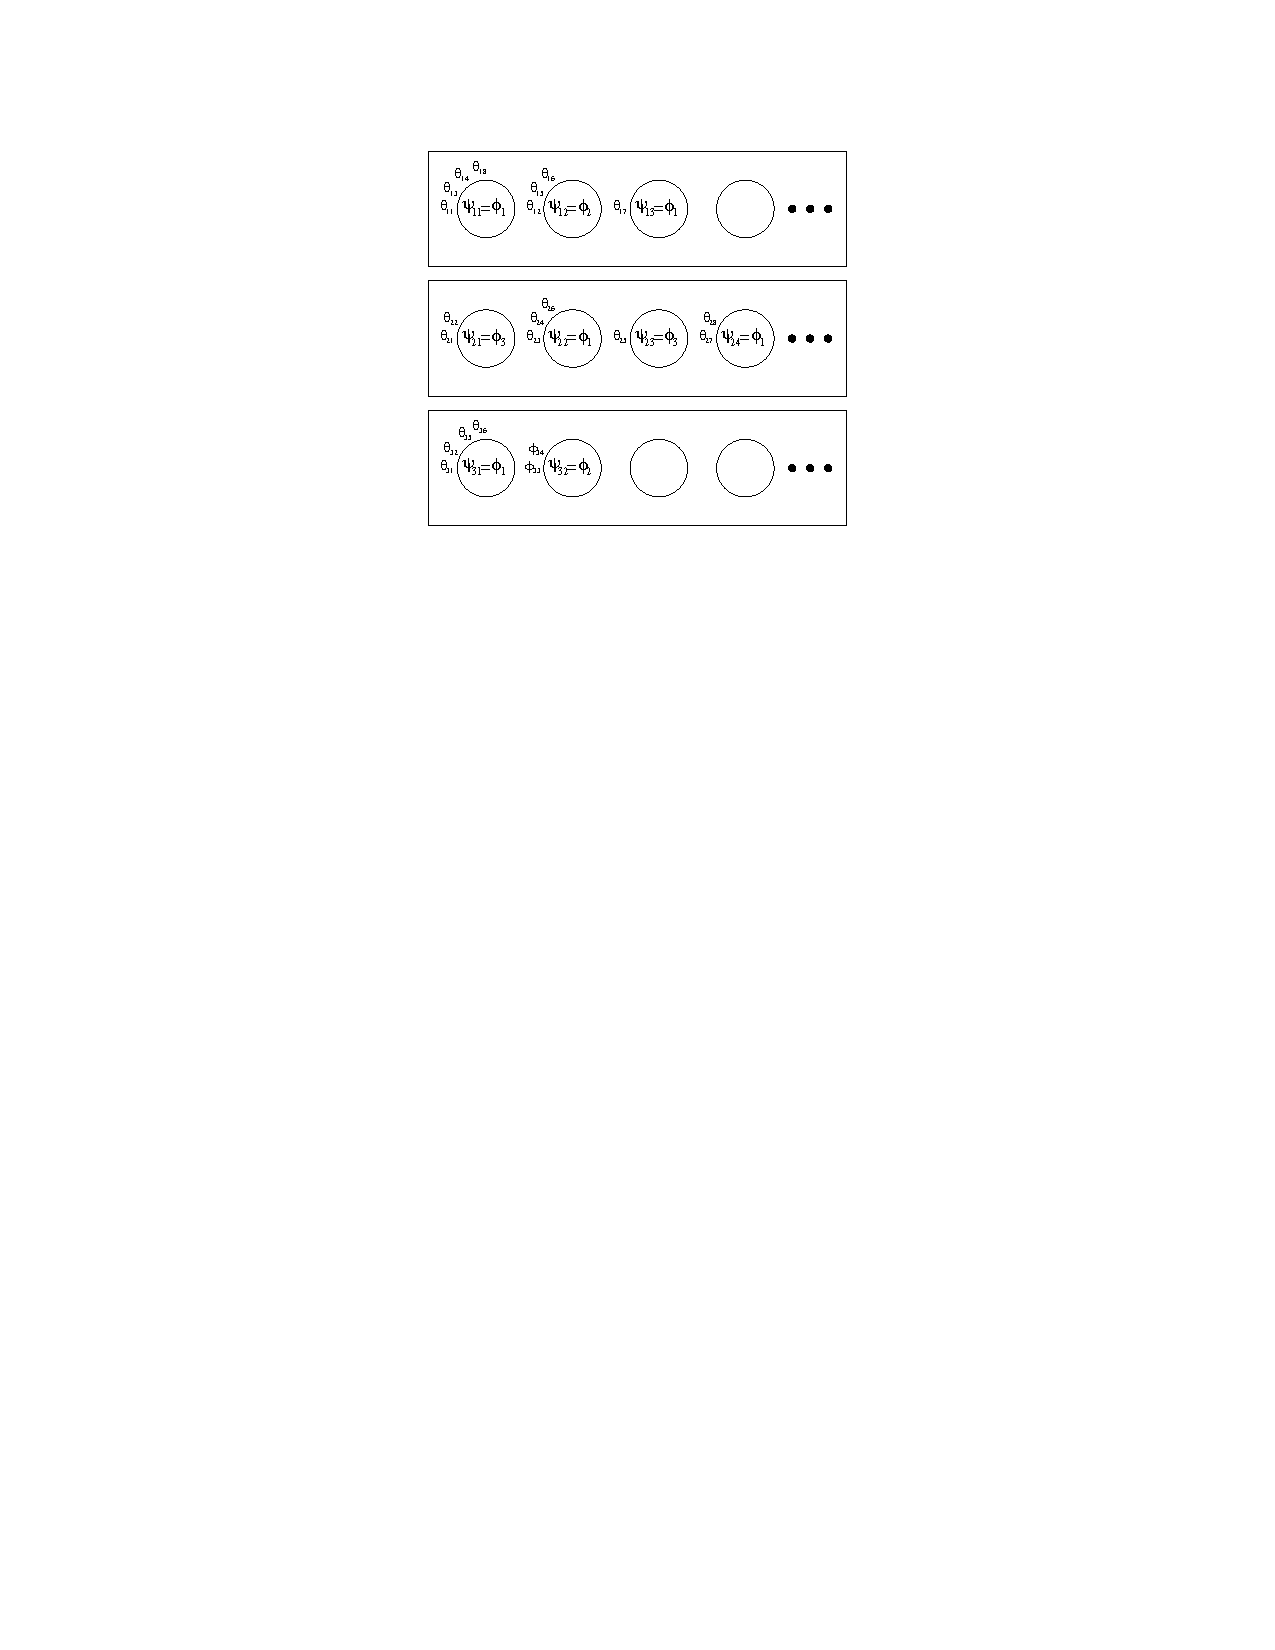
\includegraphics[height=.5\textheight]{ChineseRestaurantFranchise.pdf}
}

\itemb
\item Within each restaurant, you have the usual CRP
\item At each table, a single dish is served
\item Dishes are drawn from a global menu, via a {\em separate} CRP
\item Tables in different restaurants can share the same dish
\iteme

\end{frame}



\section*{Summary}

\begin{frame}{Summary}

  % Keep the summary *very short*.
  \begin{itemize}
  \item Chinese Restaurant Process
   \itemb
   \item Induces a prior over partitions of customers to tables
   \iteme
  \item Dirichlet Process
   \itemb
   \item Associates a mixture component with each table
   \item Numerous extensions, e.g. hierarchical DP
   \iteme
  \item Ewens' Sampling Formula
   \itemb
   \item Distribution of table occupancies
   \item Occurs in population genetics \& ecology
   \iteme
  \end{itemize}

\end{frame}


\end{document}
